\documentclass{article}
\usepackage{amssymb}
\usepackage{amsmath}
\usepackage{graphicx}
\usepackage[utf8]{inputenc}
\usepackage[text={6.5in,8.5in}]{geometry}
\usepackage{listings}
\usepackage{hyperref}
\usepackage{subcaption}
\usepackage{pdflscape}
\usepackage{adjustbox}

\lstset{language=Python, numbers=left, tabsize=2, xleftmargin=5.0ex}

\title{Parallel Implementations of the\\Fast Fourier Transform}
\author{Ari Bruck\\Eric Addison }
\date{EE382V Parallel Algorithms - Summer 2017}

\begin{document}

\maketitle

\section{Introduction}
The Fast Fourier Transform (FFT) has been described as perhaps the most important algorithm of our lifetime. The FFT moniker actually refers to a class of algorithms that can compute the Discrete Fourier Transform (DFT) in better than the naive $\mathcal{O}(n^2)$ complexity. FFTs are used across a wide range of disciplines, from audio compression to astrophysics, and have a critical role in a substantial amount of the technology we enjoy today.

For this project, our goal was to explore the classic Cooley-Tukey FFT algorithm in its sequential form, and to parallelize it using Cilk and Cuda. To this end, we have implemented the FFT in several ways, including:
\begin{itemize}
    \item sequential $\mathcal{O}(N^2)$ DFT in C++
    \item sequential recursive FFT in C++
    \item sequential iterative FFT in C++
    \item parallel recursive FFT in C++ with CILK
    \item parallel iterative FFT in C++ with CILK
    \item parallel iterative FFT in C++ with CUDA
\end{itemize}

The code for this project is available on github at: 
\begin{center}
\url{https://github.com/ericaddison/Parallel\_Algs\_Term\_Project/}
\end{center}


\section{Fourier Decomposition}
A common technique in physics and mathematics for solving complicated problems is to find a different way to represent the quantities involved. Familiar examples include solving a system of linear equations by arranging the coefficients in a matrix and making use of linear algebra, or determining the result of interactions in simple billiard-ball style dynamic systems using conservation of energy instead of sums of forces. The technique we discuss here is the process of representing a mathematical function (or signal, or time series) as a composition of sinusoids. This change of representation allows simplified solutions to problems ranging across countless disciplines, as well as a method for signal decomposition and analysis. There are four primary expressions of Fourier decomposition, depending on whether the input and output signals are continuous or discrete.

\subsection{Fourier Series}
The Fourier Series is the simplest form of Fourier decomposition to understand. Consider a periodic function $x(t)$. Recall that a function is periodic if there exists a number $T\in \mathbb{R}$ such that $x(t+nT) = x(t)$ for all $n \in \mathbb{Z}$. The Fourier Series associated with this function is given by
\[
x(t) = \sum_{k=0}^{\infty}(a_k \sin(k\omega_0t) + b_k \cos(k\omega_0t))
\]
The Fourier coefficients $a_k$ and $b_k$ describe how much each frequency $k\omega_0$ contributes to the function. The fundamental angular frequency $\omega_0$ is determined by the period, i.e. $\omega_0 = 2\pi/T$. It is common to express the series as a single summation over complex sinusoids instead of over sines and cosines, i.e.
\[
x(t) = \sum_{k=-\infty}^{\infty}c_k e^{ik\omega_0t}
\]
The simplification to one set of coefficients $c_k$ is offset by an extension of the summation variable $k$ to start from $-\infty$ instead of $0$. The is the well known \textbf{Fourier Series}, which, given a continuous function $x(t)$, is a discrete function of the frequency multiplier $k$. The coefficients $c_k$ are given by the inner product of $x(t)$ with a particular frequency $\exp{(-ik\omega_0t)}$, e.g.
\[
X[k] = c_k = \langle x(t),e^{ik\omega_0t}\rangle = \dfrac{1}{T}\int_{0}^{T} x(t) e^{-ik\omega_0t} dt 
\]

\subsection{Fourier Transform}
The next step is to allow the period $T$ grow to infinity. In this case, the fundamental frequency $\omega_0$ shrinks toward zero. By holding certain quantities constant in this limit, what was previously a summation becomes an integration, and we can now represent arbitrary (not necessarily periodic) functions by the Fourier integral:
\[
x(t) = \dfrac{1}{2\pi}\int_{-\infty}^{\infty}X(\omega) e^{i\omega t}d\omega
\]
The \textbf{Fourier Transform} refers to the coefficients, which have become a continuous function $X(\omega)$, determined again by the inner product:
\[
X(\omega) = \langle x(t),e^{i\omega t}\rangle = \int_{-\infty}^{\infty} x(t) e^{-i\omega t} dt 
\]
This remarkable formula now allows us to decompose any function $x(t)$ into the superposition of an infinite number of complex sinusoids. This is useful in a large number of technical fields, not least of which is mathematics: the special case of transforming the derivative of a function results in changing a differential equation into an algebraic equation. For this reason, Fourier transforms are a fundamental tool in the solutions of partial differential equations. In this case, both the input signal and the output transform are continuous functions: wonderful for theoretical calculations, but not easy to implement in a digital computer.

\subsection{Discrete Time Fourier Transform}
Next, let's turn our attention to a function that has been discretely sampled. A sampled function (or signal) can be thought of as a continuous function that is only defined at multiples of the sampling period $T$. For example, the sampled version of a continuous function $x(t)$ can be written
\[
x_s(t) = \sum_{n=-\infty}^{\infty}x(t)\delta(t-nT) \sim x(nT) \sim x[n]
\]
where $\delta (t)$ is the Dirac delta function. The twiddles signify a common ``abuse of notation". This modification of the input signal can be used to form discrete versions of the previous two Fourier decompositions we have discussed. The \textbf{Discrete Time Fourier Transform}, or DTFT, which has broad application in Electrical and Computer engineering, is defined by sampling the signal in time (or whatever the input variable represents), but keeping the frequency variable continuous. The DTFT transform pair is given by the inverse transform:
\[
x[n] = \dfrac{1}{2\pi}\int_{-\infty}^{\infty}X(e^{i\omega})e^{i\omega n}d\omega
\]
and forward transform
\[
X(e^{i\omega}) = \sum_{n=-\infty}^{\infty}x[n]e^{-i\omega n}
\]

\subsection{Discrete Fourier Transform}
The final version of Fourier decomposition is the last permutation of continuous and discrete functions we have available: discrete time and discrete frequency. This turns out to be equivalent to sampling in both the time and frequency domains. This final transform is called the \textbf{Discrete Fourier Transform}, or DFT, and is particularly useful because it can easily be implemented in a digital computer. The definition of the transform pair for a discrete signal of finite length $N$ is given by:
\[
x[n] = \dfrac{1}{N}\sum_{k=0}^{N-1}X[k]e^{i2\pi n k /N}
\]
and
\[
X[k] = \sum_{n=0}^{N-1}x[n]e^{-i2\pi n k /N}
\]
Note here that we choose to write out the angular frequency explicitly, i.e. $\omega_k \rightarrow 2\pi k/N$, as is typical when expressing the DFT, as this makes important properties of the DFT more obvious (for example periodicity of the DFT). A formulation of Fourier decomposition that can be easily implemented on a computer is quite useful, and has found countless applications across various fields, for example:
\begin{itemize}
    \item Spectral analysis of communication signals
    \item Digital implementation of frequency domain solutions to PDEs
    \item Frequency filtering of audio signals
    \item Large polynomial multiplication
    \item Analysis of the Cosmic Microwave Background
    \item etc...
\end{itemize}



\subsection{DFT Implementation}
\label{DFT_implementation}
The DFT can be expressed in pseudo code as:
\begin{lstlisting}
DFT(x)
N = x.length
v = -i*2*pi/N     // i == imaginary unit
for k in 1..N
    X[k] = 0
    for j in 1.. N
        X[k] += x[j] * exp(v*k)
\end{lstlisting}
Since this implementation contains two full-length \texttt{for} loops, the time complexity is $\mathcal{O}(N^2)$.


\subsection{Signal Decomposition}
We now show two examples of using the DFT to decompose an input signal into its constituent sinusoidal frequencies. Each two-panel image (figures \ref{decomp1} and \ref{decomp2}) shows an input signal on the left, and the DFT of that signal on the right. We plot the amplitude of each DFT sample, as is typical with spectral displays. The amplitude display shows how the sinusoids at different frequencies have contributed to the composite signal. The signals shown have the form:
\[
x_1[n] = \sin(2\pi f_1 n) + 0.5\cos(2\pi f_2 n) +  0.2\cos(2\pi f_2 n + \pi/4)
\]
and
\[
x_2[n] = U +  0.2\sin(2\pi f_0 n)
\]
Where $U$ is a uniform random variable $U\sim \mathcal{U}(-0.5, 0.5)$, $f_0 = 0.25$Hz, $f_1=0.001$Hz, $f_2=0.2$Hz, and $f_3=0.4$Hz. There is an implicit sampling rate of $T_s = 1$s.

\begin{figure}
    \centering
    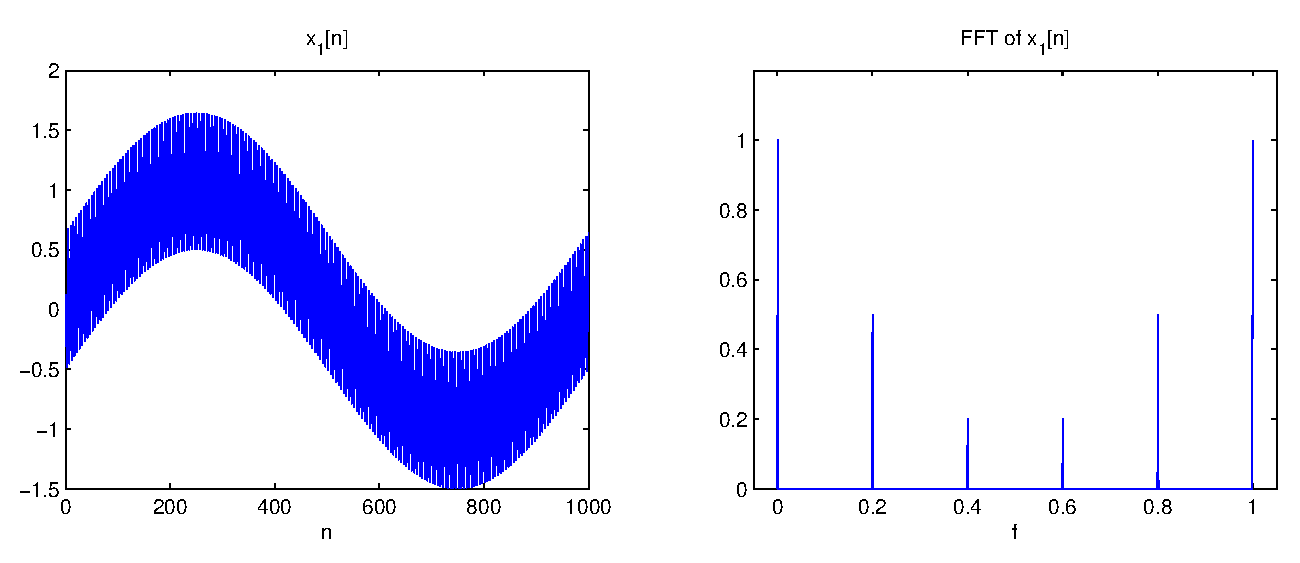
\includegraphics[scale=0.6]{./img/sins.eps}
    \caption{The function $x_1[n]$ (left) and its DFT (right). Notice that the DFT shows spikes at the frequency of each sinusoid in the signal, and also at the mirrored location $f'=f_{max}-f$, where $f_{max}=1/T_s$. Because of this mirroring, unique frequencies can only be represented up to $f_N=1/(2T_s)$, which is known as the Nyquist frequency.}
    \label{decomp1}
\end{figure}
\begin{figure}
    \centering
    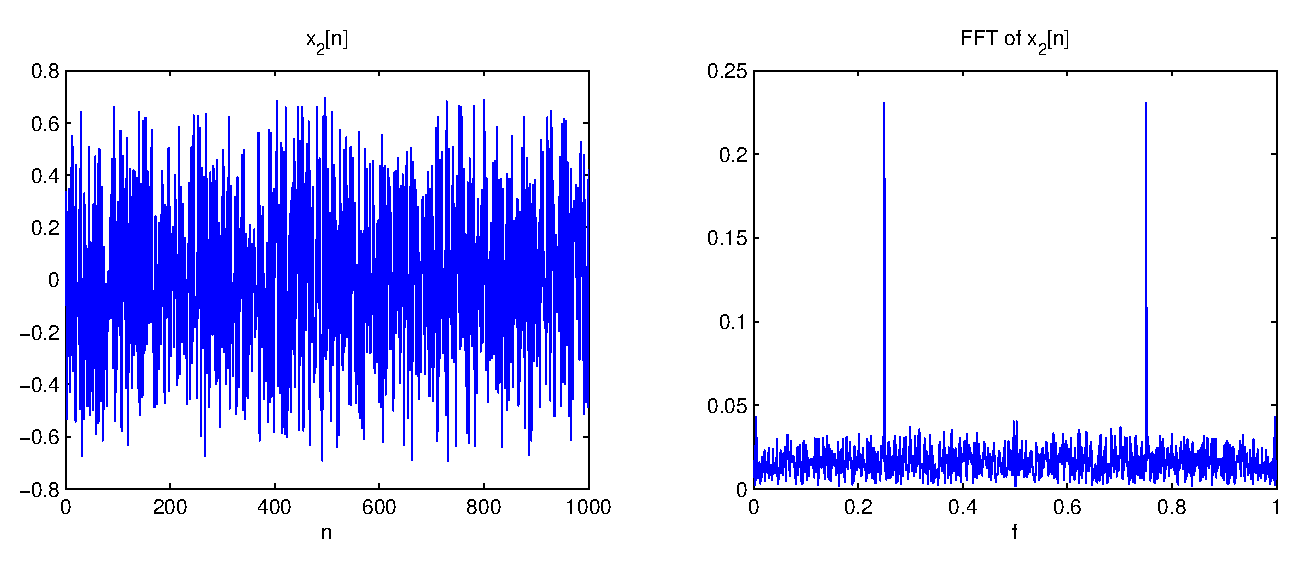
\includegraphics[scale=0.6]{./img/random.eps}
    \caption{The function $x_2[n]$ (left) and its DFT (right). Notice that the DFT show the spike at $f_0=0.25$Hz, and its mirror. This illustrates one of the advantages of the DFT: though it was difficult to spot the sinusoidal oscillation in the time-domain signal (left), it sticks out quite clearly in the frequency domain (right).}
    \label{decomp2}
\end{figure}


\subsection{Symmetry in the FFT Algorithm}
\label{fftSymmetry}
The symmetry seen in the Cooley-Tukey FFT algorithm (lines 11 and 12 in the code listing from section \ref{fftRecursive}) can be explained by exploiting symmetry of the DFT:
\begin{align*}
X[k+N/2] &= \sum_{n=0}^{N/2-1}x_e[n]e^{-i2\pi n (k+N/2) /(N/2)} + e^{-i2\pi (k+N/2)/N}\sum_{n=0}^{N/2}x_o[n]e^{-i2\pi n (k+N/2) /(N/2)}\\
&=\sum_{n=0}^{N/2-1}x_e[n]e^{-i2\pi n k/(N/2)}e^{-i2\pi n} + e^{-i2\pi k/N}e^{-i\pi}\sum_{n=0}^{N/2-1}x_o[n]e^{-i2\pi n k/(N/2)}e^{-i2\pi n}\\
&= \sum_{n=0}^{N/2-1}x_e[n]e^{-i2\pi n k/(N/2)} - e^{-i2\pi k/N}\sum_{n=0}^{N/2-1}x_o[n]e^{-i2\pi n k/(N/2)}\\
&= X_e[k] - e^{-i2\pi k/N}X_o[k]
\end{align*}


\section{The Fast Fourier Transform}
An FFT algorithm computes the DFT of a signal in better than $\mathcal{O}(N^2)$ time. See Appendix \ref{theoryAppendix} for a review of the theory related to Fourier decomposition. 

The naive implementation of the DFT, as shown in section \ref{DFT_implementation}, has time complexity $\mathcal{O}(N^2)$. This can be done more efficiently with a divide and conquer approach. Consider the original equation for the DFT:
\[
X[k] = \sum_{n=0}^{N-1}x[n]e^{-i2\pi n k /N}
\]

Now split the sum in two, one with the even entries of $x[n]$ and one with odd:
\begin{align*}
X[k] &= \sum_{n=0}^{N-1}x[n]e^{-i2\pi n k /N}\\
&= \sum_{n=0}^{N/2-1}x[2n]e^{-i2\pi (2n) k /N} + \sum_{n=0}^{N/2-1}x[2n+1]e^{-i2\pi (2n+1) k /N}\\
&= \sum_{n=0}^{N/2-1}x[2n]e^{-i2\pi (2n) k /N} + e^{-i2\pi k/N}\sum_{n=0}^{N/2-1}x[2n+1]e^{-i2\pi (2n) k /N}\\
&= \sum_{n=0}^{N/2-1}x_e[n]e^{-i2\pi n k /(N/2)} + e^{-i2\pi k/N}\sum_{n=0}^{N/2-1}x_o[n]e^{-i2\pi n k /(N/2)}\\
&= X_e[k] + e^{-i2\pi k/N}X_o[k] \tag{*} \label{evenOdd} 
\end{align*}
where $x_e[n]$ and $x_o[n]$ are the signals formed by collecting the even and odd entries of $x[n]$, and $X_e[k]$ and $X_o[k]$ are the $N/2$ point DFTs of $x_e[n]$ and $x_o[n]$, respectively. This form of the DFT equation suggests that a divide and conquer strategy could be applied. We examine this now.

\subsection{Divide and Conquer DFT Complexity}
From an algorithmic perspective, the even-odd split of the DFT equation strongly suggests the use of recursion. What is the complexity in this case? Suppose the complexity of computing the DFT in this manner is given by $T(N)$, and that $N=2^{h}$, then
\begin{align*}
T(N) &= T(N/2) + T(N/2) + \mathcal{O}(N/2)\\
&= (T(N/4) + T(N/4) + \mathcal{O}(N/4)) \\
&\quad + (T(N/4) + T(N/4) + \mathcal{O}(N/4)) + \mathcal{O}(N/2)\\
&= 4T(N/4) + 2\mathcal{O}(N/4) + \mathcal{O}(N/2)\\
&= ...\\
&= 2^h T(1) + \sum_{i=1}^{h}2^i \mathcal{O}(N/2^i) \tag{**} \label{bottomOfTree}\\
&= N\mathcal{O}(1) + \sum_{i=1}^{\log N} \mathcal{O}(N)\\
&= \mathcal{O}(N) + \mathcal{O}(N\log N)\\
&= \mathcal{O}(N\log N)
\end{align*}
A few key properties were used in this equation. The calculation started by writing $T(N)$ as the sum of the time it would take to compute the even and odd side DFTs, plus an extra factor of $\mathcal{O}(N/2)$ for the multiplication of the so called ``twiddle factor" that precedes the odd-side DFT in the equation marked \ref{evenOdd}. Continuing to expand the $T(N)$ terms by walking down the implicit binary tree (splitting $h$ times) leads to equation \ref{bottomOfTree}. The DFT of a single value is just the value itself, so the complexity of $T(1) = \mathcal{O}(1)$. By making use of the fact that $h = \log N$, the next lines follow directly. 

We can see now that the complexity of this divide and conquer algorithm is $T(N) = \mathcal{O}(N\log N)$. This algorithm is known as the Tukey-Cooley algorithm, named after the authors of its modern incarnation J.W. Cooley and John Tukey, though it was known as early as 1805 by none other than Carl Friedrich Gauss. The Tukey-Cooley algorithm is part of a class of algorithms known as \textbf{Fast Fourier Transforms}, or FFTs, which share the common trait of expressing a DFT such that it can be computed in $\mathcal{O}(N\log N)$ time. Other FFT algorithms exist, though we do not explore them here.

As a side note, there is nothing magic about splitting the DFT problem into two pieces, as we did above. This approach is known as the radix-2 Decimation in Time (DIT) Tukey-Cooley FFT. For any other positive integer $b$, with $N = b^h$, we could perform the same type of DFT splitting (called the radix-b DIT FFT):
\[
X[k] = \sum_{s=0}^{b-1} \left( e^{-i2\pi s k/N}\sum_{n=0}^{N/b-1}x[bn+s]e^{-i2\pi n k /(N/b)} \right),
\]
which would evaluate to have the same time complexity $\mathcal{O}(N\log N)$. A more advanced FFT algorithm might split the DFT calculation differently at each level of the recursion tree, allowing efficient computation for general composite values of $N$. In this project, however, we focus on the radix-2 case for $N$ a power of 2.

\subsection{Recursive Implementation}
\label{fftRecursive}
A pseudo code implementation of the recursive Tukey-Cooley algorithm is straight forward and has $T(n) = \mathcal{O}(N \log N)$:
\pagebreak
\begin{lstlisting}
FFT_REC(x)
    N = x.length
    if N <= 1
        return
    v = -i*2*pi/N     // i == imaginary unit
    for s in 2..log(N)
        E = FFT_REC( [x[2*n] for n = 0..N/2-1] )
        O = FFT_REC( [x[2*n+1] for n = 0..N/2-1] )
        for j in 0..N/2-1
            w = exp(v*j)
            x[2*j] = E[j] + w*O[j]
            x[2*j+N/2] = E[j] - w*O[j]
    return x
\end{lstlisting}

The symmetry seen in lines 11 and 12 arise from the symmetry present in the DFT. For a mathematical explanation of the symmetry of lines 11 and 12, see section \ref{fftSymmetry}. 


\subsection{Iterative Implementation}
Running the recursive FFT algorithm of a vector of length 8 shows the following execution diagram. The first element is combined with the fourth and the second with the sixth. Those products are then combined and create what was termed the Even side of the recursive algorithm. This observation is going to be used to create an iterative FFT algorithm. The leaves of the recursion tree show a particular order in which the initial elements are permuted. If we could shuffle the input the match this ordering in another way, then we could avoid the recursive calls that work down the tree and start from the bottom up.

\begin{figure}[h]
\center
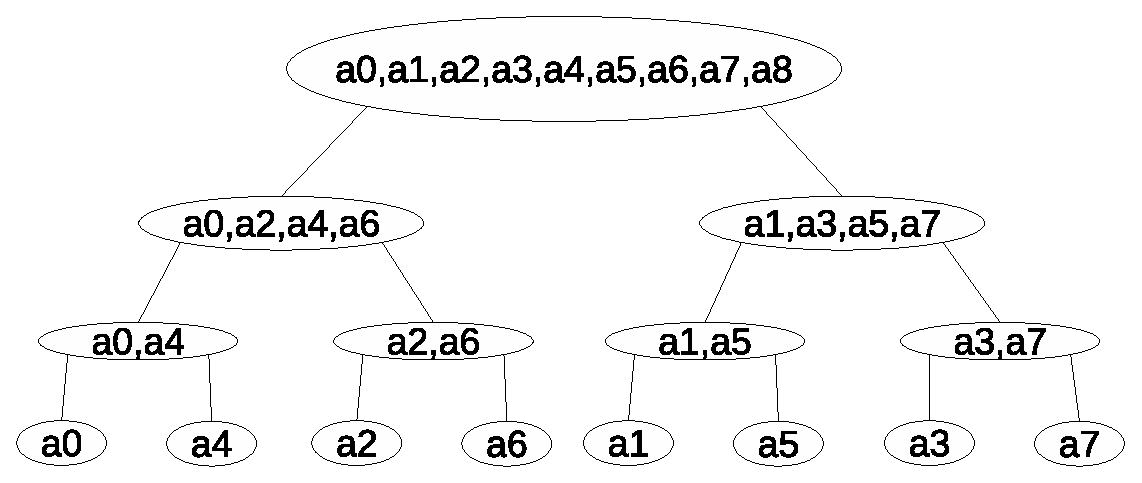
\includegraphics[scale=0.5]{img/recursive_fft_execution.eps}
\caption{Execution path of the recursive FFT algorithm given an input vector a with 8 entries}
\end{figure}

If the 8-element vector above is taken as an example, the desired order is (0,4,2,6,1,5,3,7). In binary, the original input \texttt{(000,001,010,011,100,101,110,111)} becomes \texttt{(000,100,010,110,001,101,011,111)}. A bit-reversal will accomplish this transformation, e.g. for an array index with $d$ bits,
\[
k = b_{d-1}b_{d-2}b_{d-3}...b_0 \rightarrow b_0b_1...b_{d-2}b_{d-1} = k'
\]

The \texttt{Bit-Reverse()} function performs the reordering by:
\begin{lstlisting}
Bit-Reverse(x)
    y = empty vector
    for k in 0..x.length-1
        k2 = reverse_bits(k)
        y[k] = x[k2]
    return y
\end{lstlisting}

Therefore \texttt{Bit-Reverse()} is used to unroll the recursive execution and transform it into an iterative one. The iterative algorithm is also $T(n) = \mathcal{O}(n * log(n))$ similar to the recursive algorithm.

A pseudo code implementation of the iterative Tukey-Cooley algorithm is:
\begin{lstlisting}
FFT_ITER(x)
    Bit-Reverse (x)
    N = x.length
    for s in 1..log(N)
        m = 2^s
        wm = exp(-i2*pi/m)
        w = 1
        for j in 0..(m/2-1)
            for k in j..(n-1) by m
                t = w * x[k + m/2]
                u = x[k]
                x[k] = u + t
                x[k + m/2] = u - t
            w = w*wm
    return x
\end{lstlisting}

\subsection{FFT Performance}
The relative performance of the sequential algorithms discussed above are shown in figure \ref{seqTimes}. These include the plain DFT, recursive and iterative Cooley-Tukey FFT, and the numpy FFT function. The plot is logarithmic along both axes. Clearly the DFT performs the worst. Our iterative and recursive implementations are similar, with the iterative algorithm performing about two times better on average. The numpy implementation is far better, performing about 10 times better on average than our recursive implementation. The similar slopes of the three FFT algorithms confirm that they have the same asymptotic complexity, which we know is $\mathcal{O}(N\log N)$.

\begin{figure}[h!]
\centering
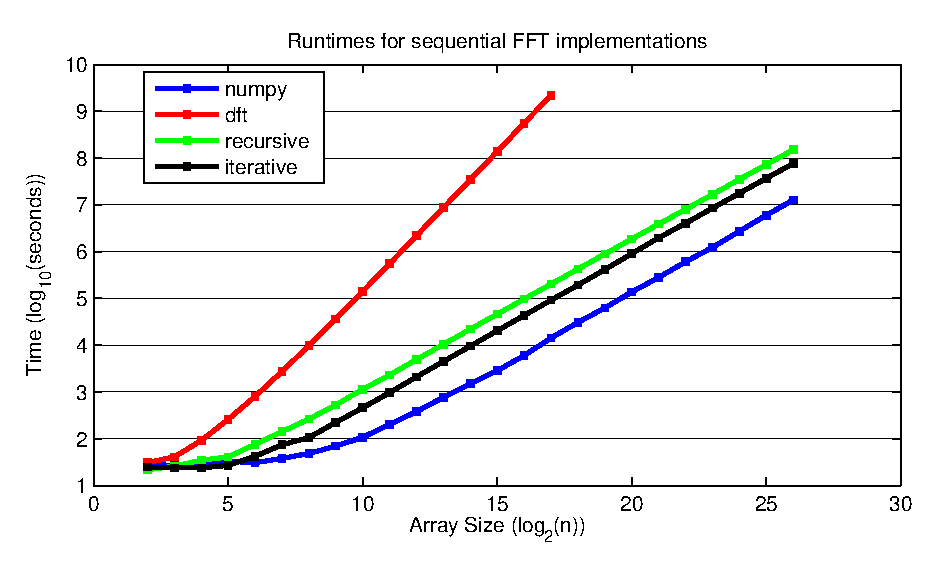
\includegraphics[scale=0.9]{img/seqRuntimes.eps}
\caption{Runtimes for the sequential algorithms.}
\label{seqTimes}
\end{figure}

\section{Parallelization of the FFT}
Converting the Iterative FFT algorithm into a parallel implementation is straight-forward. At each of the $log(N)$ levels, there will be work that can be done in parallel. The figure below shows the combinational circuit with three stages of work, where the work done in each stage can be done in parallel.

As shown in the following figure, and seen from the previous recursion tree, a parallel implementation of the FFT algorithm can be computed in $\mathcal{O}(\log N)$ time with $N$ processors. Since no extraneous work is performed, the work complexity is $\mathcal{O}(N\log N)$, so this is a work-optimal algorithm. 

\begin{figure}[h]
\center
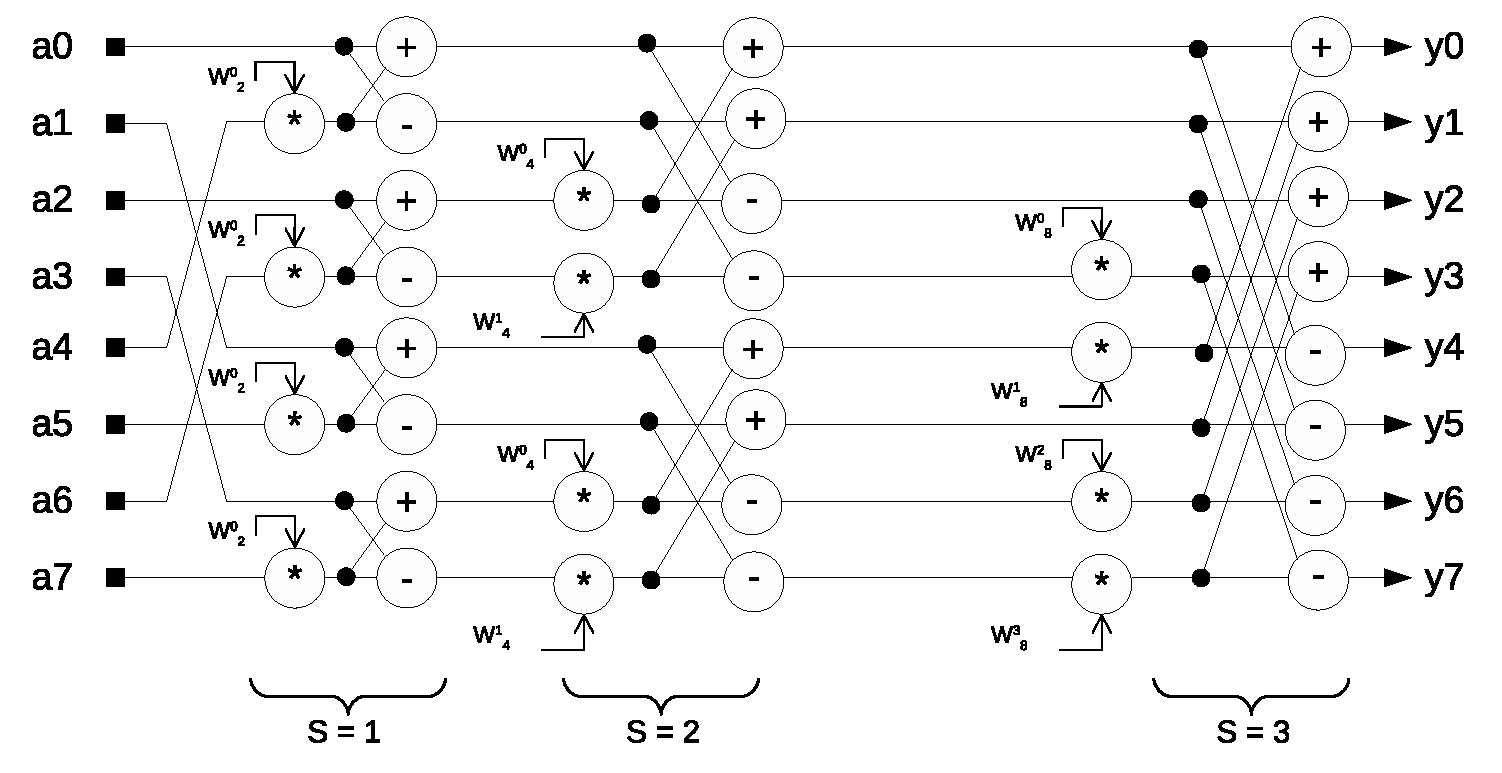
\includegraphics[scale=0.45]{img/parallel_fft_circuit.eps}
\caption{Combinational circuit Parallel-FFT that computes the FFT, here with $n$=8 inputs. The stages are labeled to correspond with the outermost loop of \texttt{FFT\_ITER()}. An FFT on $N$ inputs can be computed in $O(\log N)$ depth with $O(N \log N)$ elements}
\end{figure}

\section{Cilk}

See Appendix \ref{cilkAppendix} for history and background of cilk.

\subsection{Cilk Implementation: Recursive}

The classic Cooley-Tukey FFT algorithm makes use of recursion to reduce computation time of FFT decomposition by splitting up the even and odd terms. Cilk parallelism can be exposed in recursive algorithms with ease by utilizing the \texttt{cilk\_spawn} and \texttt{cilk\_sync} keywords. Since the even and odd terms of the FFT are independent a CPU with sufficient resources will be able to compute these in parallel given cilk’s spawn routines. When both spawned children are done they must be synced to ensure coherent programming order.

From a programming point of view, cilk is a very easy tool for the programmer to use since the recursive routine can first be written without any cilk constructs. When functional correctness is established, the cilk keywords may be introduced.

The merging step that occurs after the divide and conquer steps are complete can also expose parallelism to cilk. In our implementation this step is called via the \texttt{cilk\_combine()} function. Cilk spawns two threads of \texttt{cilk\_combine()} with arrays of half the size. When the sub-arrays reach below a certain threshold of \texttt{cilk\_max\_recombine}, the \texttt{cilky\_combine()} function is called. This function uses the \texttt{cilk\_for} construct to parallelize work.

From a parallel algorithms perspective it is interesting to note the performance impact of the value of \texttt{cilk\_max\_recombine}. Figure \ref{cilk_max_recombine} shows that as the number of elements of the FFT grows, there is a noticeable performance gap between the two cilk recursive runs where the only change is in the value of \texttt{cilk\_max\_recombine} (value of 1 vs. 128). A value of 128 represents fewer threads processing more values in \texttt{cilky\_combine()} as compared to a value of 1 where more threads are processing fewer elements in parallel. This is akin to the cascaded parallel algorithm technique of splitting up the groups of elements a certain way to achieve a work-optimal solution. 

It should be noted that the recursive solution is still of work-complexity $\mathcal{O}(n * log(n))$ as the algorithm is not changed. However, the cilk constructs expose potential parallelism which means that overall running time is decreased given system resources. 



\subsection{Cilk Implementation: Iterative}
The introduction of the \texttt{cilk\_for} construct allows for loops with independent operations to run in parallel. Replacing one \texttt{for} with a \texttt{cilk\_for} in the \texttt{cilk\_transform\_iter()} function results in a dramatic performance boost as can be seen in the graph of figure \ref{iterative_fft}. 
Similarly to the recursive cilk implementation, the cilk iterative algorithm is still of the same complexity, $W(n) = \mathcal{O}(n * log(n))$, but is faster due to the exposed parallelism. 

\subsection{Cilk Analysis}
As can be seen in the graph of figure \ref{fft_cilk_cpp}, the performance differences between the five different algorithms becomes clear when processing at least 2\textsuperscript{10} elements. The non-cilk C++ recursive algorithm is the slowest performance-wise. The recursive recursive  implementation that uses a value of \texttt{cilk\_max\_recombine} value of 1 is faster than the non-cilk version, but not by much. An interesting observation is that the cilk recursive algorithm with a \texttt{cilk\_max\_recombine} value of 128 is faster than the version that uses a value of 1 for all values save some outliers. In fact, it is close to \( \frac{2}{3} \) the completion time of the \texttt{cilk\_max\_combine} value of 1.

\begin{figure}
\center
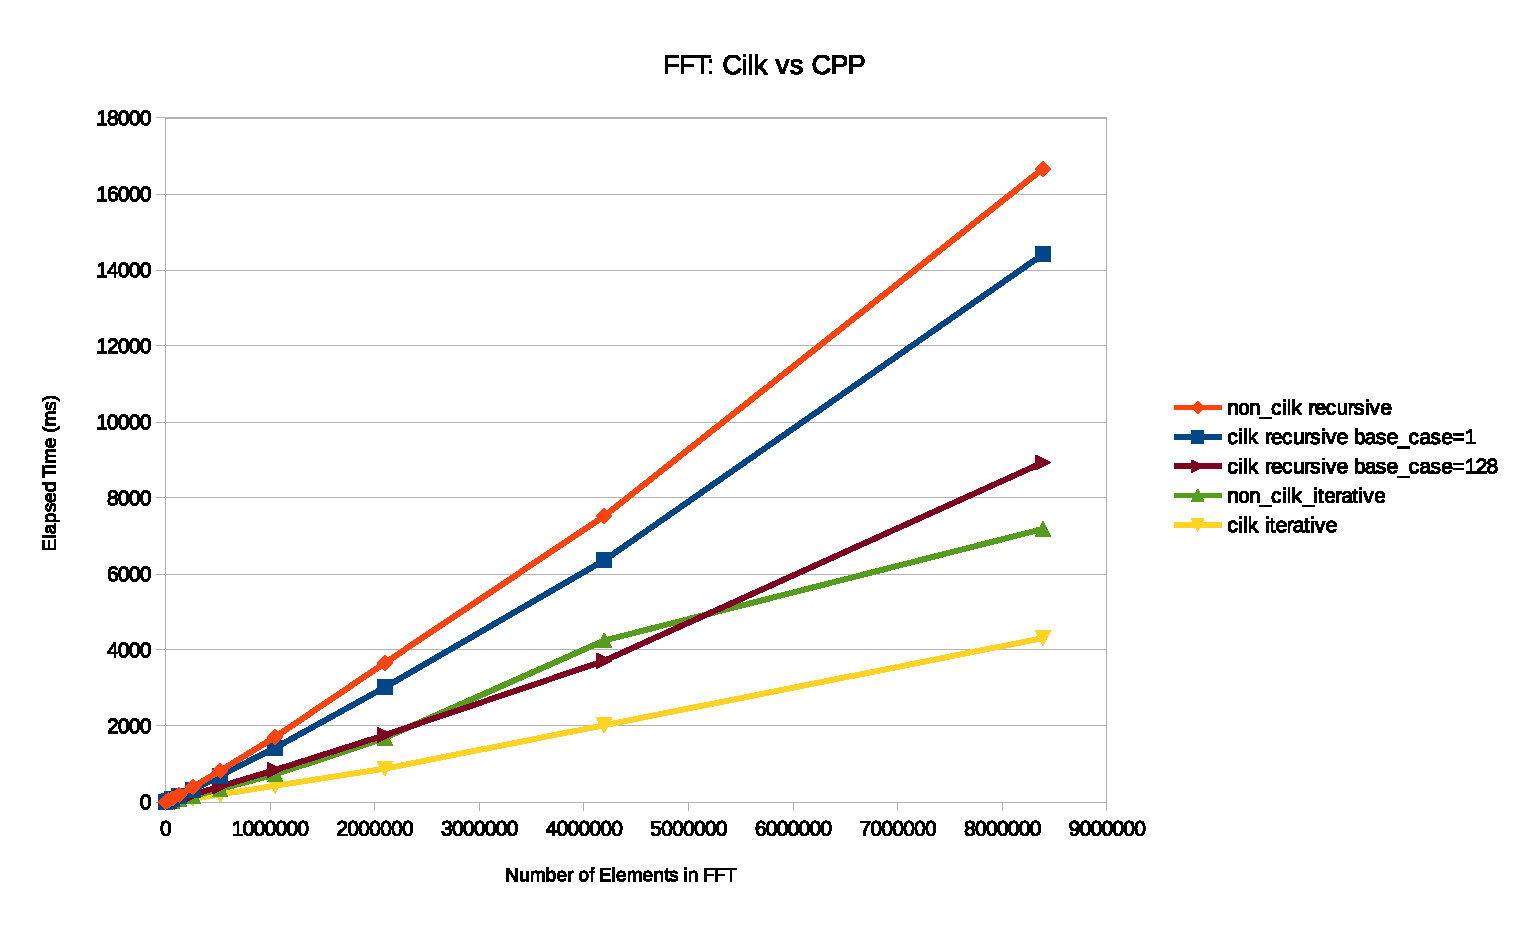
\includegraphics[scale=0.8]{img/fft_cilk_cpp.eps}
\caption{Graph comparing the performance of all FFT algorithms, cilk and C++} 
\label{fft_cilk_cpp}
\end{figure}

Moreover, the iterative cilk implementation is by far the highest performing algorithm. It is about 1.6x times faster than the non-cilk version for large values. Another observation worth noting is that the iterative non-cilk solution is ~2.3x faster than its non-cilk version. This relationship is similar between the cilk iterative implementation and the recursive cilk \texttt{cilk\_max\_recombine}=128 solution (~2x performance gains), while it grows to as much as ~3.3x as compared to the recursive cilk \texttt{cilk\_max\_recombine}=1 solution . 

Cilk does provide built-in ways to adjust the “grain-size” of the threads. This was not used in this project; however, from the curves of the graph in figure \ref{cilk_max_recombine} it is obvious that a lot of performance improvement can be gained with calibration of the number of threads cilk uses. 

The parallelism gained by cilk comes at the cost of memory (space complexity) usage. Inherently, it is very difficult to measure stack usage by cilk since it manipulates the stack so much to achieve parallelism that any attempts to trace stack usage affects cilk performance negatively. However, heap usage is easy to measure using the program profiling tool Valgrind with the heap profiler massiff. As can be seen from images in figure \ref{fig:masiff}, the iterative cilk solution that uses the \texttt{cilk\_for} construct does not use much more heap space than the non-cilk iterative one. This may be due to cilk’s internal vectorization instead of the spawn/sync mechanism. The recursive cilk solution uses more heap space than the non-cilk version (~41MB vs. ~28MB). 



\section{Cuda}
See appendix \ref{cudaAppendix} for a review of the Cuda parallel processing framework.
\subsection{Cuda Implementation: Iterative}
The iterative form of the FFT algorithm is well suited for execution on a GPU. The strategy will be to treat each executing thread as single entry in the array. That is, each thread is responsible for computing the FFT value of the array location given by its global index. 

Three kernels are used to perform this task: \texttt{bit\_reverse\_kernel()}, \texttt{fft\_kernel\_shared()}, and \texttt{fft\_kernel\_finish()}. The sequence of execution in the FFT computation goes like this:
\begin{itemize}
    \item Load input data from CPU to GPU
    \item call \texttt{bit\_reverse\_kernel()} to perform array index bit-reversal in global memory
    \item call \texttt{fft\_kernel\_shared()} to perform the partial FFT using shared memory
    \item loop over \texttt{fft\_kernel\_finish()} to finish the FFT in global memory
    \item Retrieve data from GPU memory to CPU
\end{itemize}

This implementation computes all the partial FFTs in shared memory. That is, due to the thread block-size restriction of 1024 threads, this approach was not able to continue with shared memory after the FFT 1024-point FFT has been performed. The limitations were that thread synchronization during kernel execution is limited to the threads within a block, and that threads from neighboring blocks cannot access each other's shared memory.

After the shared memory computation has finished, the CPU code loops over the \texttt{fft\_kernel\_finish()} kernel, which performs one iteration of the iterative FFT loop. This was thought to be necessary so that global device synchronization could be achieved. Otherwise, since the FFT algorithm now needs to reach beyond the limits of thread-block size to continue ($m/2 > 512$), there is the potential to introduce a race condition as each block proceeds out of sync with the others. 

We implemented only the iterative FFT in cuda due to the natural programming style of GPU computations: GPUs are not ideally suited for recursive tasks. However, it is now possible to launch new grids of threads from an executing grid, where previously new grids (kernels) could only be launched from the CPU. This technique is know as Dynamic Parallelism, and enables recursive programming on the GPU. We did not explore this option, but felt it is important to mention.

\subsection{Cuda Analysis}
The performance of our cuda FFT is shown in figure \ref{cudaRuntimes}. This graph includes the numpy FFT, our cuda impementation, and the Nvidia CUFFT library function. For both cuda algorithms, full times and ``inner" times are plotted. The full time includes data transfer from CPU to GPU and back, and the inner time measures only the actual FFT computation. The total time does not include a CUDA device initialization, which can take hundreds of milliseconds.

Several interesting features are visible on the graph. Most obvious is that the CUFFT total time is significantly larger than any other of the displayed algorithms. This is due in part to the CPU/GPU memory transfer, but primarily it comes from the requirement to compute an FFT plan, which optimizes the run configuration when executing an FFT with CUFFT. For our cuda implementation, a fairly consistent amount of additional time is required for the data transfer, though the difference shrinks as $N$ increases. This is because the data transfer time is only $\mathcal{O}(N)$, while the thread saturated cuda run time is $\mathcal{O}(N\log N)$. For $N<1024$, the sequential numpy FFT outperforms either cuda implementation. A large spike in CUFFT is seen at $N=2^{12}$, which is expected based on the Nvidia published CUFFT performance tests. Between 1024 and $2^{15}$, our cuda implementation grows very slowly. After $2^{15}$, however, the cuda codes start to grow with the same slope as the numpy FFT. This makes sense: the GPUs available on Stampede are Nvidia K20m cards, which have can run a maximum of 26624 concurrent threads. The number $26624 \approx 2^{14.7}$, so the turning point in the cuda performance curve at about $2^{15}$ is expected by Brent's Scheduling Principle. Even for large values of $N$, however, our implementation performs about 10 times faster than numpy, and the built-in CUFFT is about 100x faster.

\begin{figure}
    \centering
    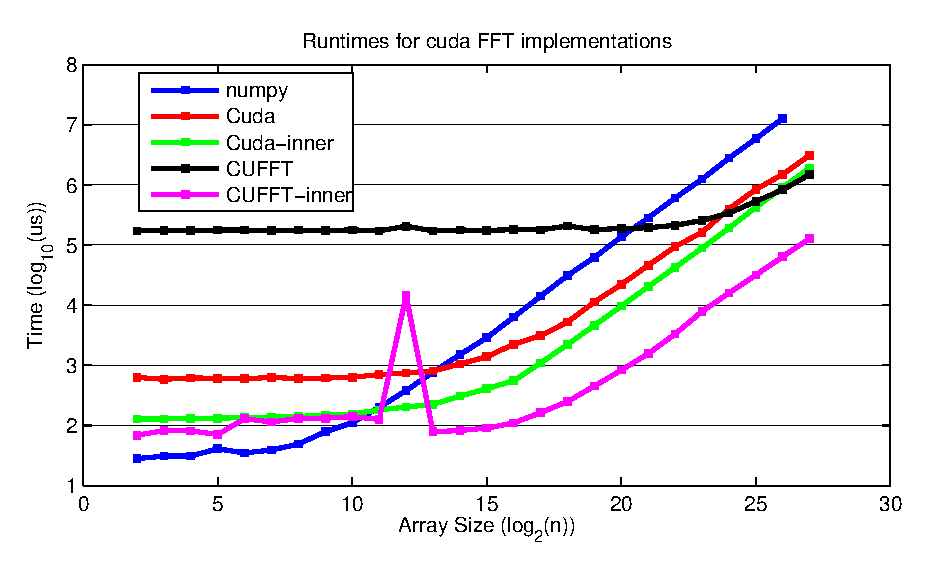
\includegraphics[scale=0.75]{img/cudaRuntimes.eps}
    \caption{Comparison of cuda FFT runtimes.}
    \label{cudaRuntimes}
\end{figure}

%\section{Analysis of Results}

\section{Conclusion}
The Fast Fourier Transform implemented in $T(N) = \mathcal{O}(N^2)$ is not tenable for large order transforms. From the above graphs it is clear that as the number of input elements grows, a better solution is needed. We have discussed two algorithms that implement the FFT. The first is the recursive solution first (re-)discovered by Cooley-Tukey. With some manipulation and bit-twiddling, the recursive algorithm can be transformed into an iterative one.

We focused on two ways to parallelize the FFT algorithm. First by using the C/C++ extension cilk, and then by implementing it on a GPU. Overall, the Cuda algorithm beat any other algorithm by several orders of magnitude. However, since the GPU is run as a device attached to the main host CPU, it suffers from the time lag needed to transfer data to and from the GPU. When processing vectors of size greater than $2^{13}$ elements, Cuda's performance even with this penalty beats the Python-Numpy implementation. 

On the other hand, Cilk was a very good contender in terms of performance as the number of elements increased. However, from our results it is obvious that the overhead of parallelism is not worth it for smaller input vectors since performance lagged as compared to the traditional C++ algorithms. For inputs with $N>2^{14}$, however, the Cilk implementations outperform the sequential algorithms. 

\section{References}
\noindent[1] Cormen, Thomas H., Charles Eric. Leiserson, Ronald L. Rivest, and Clifford Stein. "30 Polynomials and FFT." Introduction to Algorithms. Cambridge, MA: MIT, 2014. 898-925. Print.\\

\noindent[2] (Intel), Jim Sukha. "Why Is CilkTM Plus Not Speeding up My Program? (Part 1)." Intel® Software. Intel, 27 Aug. 2013. Web. 4 August 2017.\\

\noindent[3] Lee, Angela. Parallel Algorithms. N.p.: IEEE / Institute of Electrical and Electronics Engineers Incorporated, 1997. Parallel Algorithms. Washington University St. Louis, 22 Jan. 2015. Web. 4 August 2017.\\

\noindent[4] Madbmtannen. "Tutorial Cilk Plus Keywords." CilkPlus. CilkPlus/Intel, 03 Nov. 2015. Web. 4 August 2017.\\

\noindent[5] JaJa, Joseph. "Introduction to Parallel Algorithms", Addison-Wesley Professional, 1992.


\end{document}
